\documentclass[border=5pt]{standalone}
\usepackage{fontspec,xeCJK,amsmath,amssymb,tikz,graphicx}\setmainfont{Arial}\setCJKmainfont{PingFang SC}
\definecolor{ink}{HTML}{203340}\definecolor{blue}{HTML}{147E91}\definecolor{pale}{HTML}{EEF6F6}\definecolor{warm}{HTML}{FFF4E5}
\begin{document}\begin{tikzpicture}[x=1cm,y=1cm,every node/.style={text=ink,font=\fontsize{11}{14}\selectfont},box/.style={rounded corners=6pt,draw=blue!25,fill=white}]
\path[use as bounding box](0,0)rectangle(11,29);\fill[pale](0,0)rectangle(11,29);
\node[font=\fontsize{21}{25}\selectfont\bfseries]at(5.5,28.2){Diffusion Policy：生成一串动作};\node[text=blue]at(5.5,27.5){看环境 → 去噪动作序列 → 执行前段 → 再看};
\draw[box](.3,21.1)rectangle(10.7,27);\node[anchor=west,font=\bfseries\large]at(.6,26.4){A　看清当前｜§II-C、III-B};
\node at(5.5,24.4){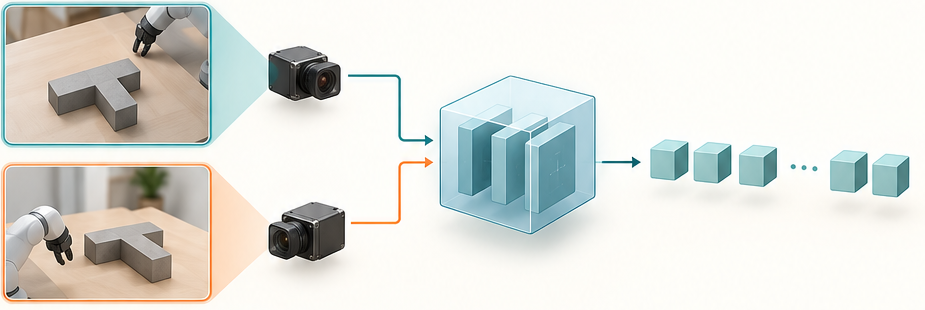
\includegraphics[width=8.8cm]{observe-art.png}};
\node at(5.5,22.6){最近 $T_o$ 帧图像 + 本体状态 $\to O_t$};\node at(5.5,21.8){视觉编码一次；条件特征供这一轮全部去噪步复用};
\draw[box](.3,14.4)rectangle(10.7,20.7);\node[anchor=west,font=\bfseries\large]at(.6,20.1){B　从噪声变动作｜§II、III-D};
\node at(5.5,18.1){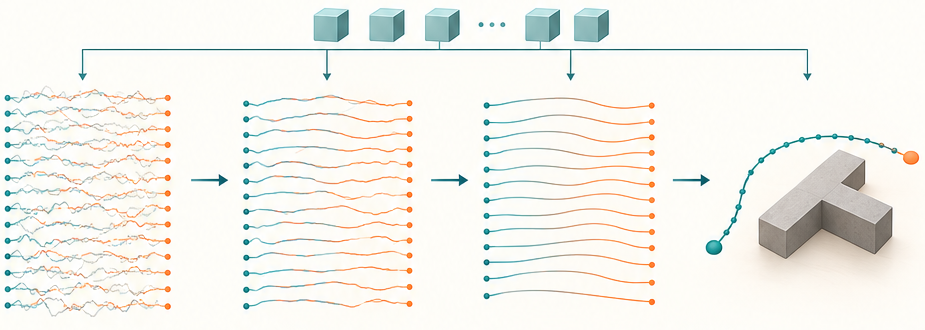
\includegraphics[width=8.8cm]{noise-art.png}};
\node at(5.5,16.3){$A_t^K\sim\mathcal N(0,I)\to A_t^{K-1}\to\cdots\to A_t^0$};
\node at(5.5,15.6){每步 C 预测同形状噪声；$O_t$ 保持不变};\node at(5.5,14.9){示例：$T_p=16,\ D_a=2\Rightarrow16\times2$ 个动作坐标};
\draw[box,fill=warm](.3,7.9)rectangle(10.7,14);\node[anchor=west,font=\bfseries\large]at(.6,13.4){C　噪声网络与训练｜§III-A、IV-D};
\node at(5.5,11.6){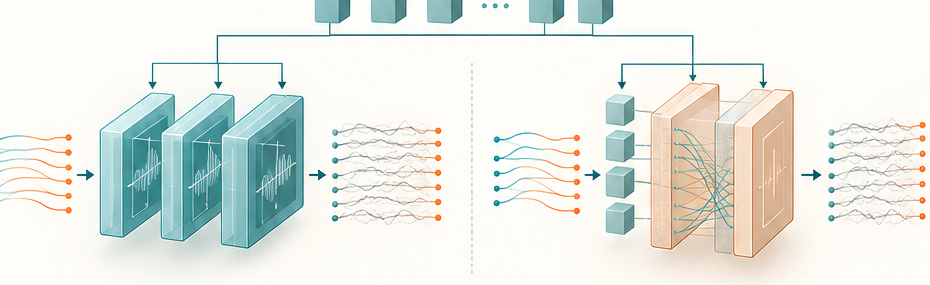
\includegraphics[width=8.8cm]{net-art.png}};
\node at(5.5,9.9){CNN：时间卷积 + FiLM；Transformer：动作读观察};
\node at(5.5,9.2){训练：示范 $A_t^0$ 加噪，监督 $\lVert\epsilon-\epsilon_\theta\rVert^2$};
\node at(5.5,8.5){同时训练视觉编码器；无奖励优化、无未来状态预测};
\draw[box](.3,.3)rectangle(10.7,7.5);\node[anchor=west,font=\bfseries\large]at(.6,6.9){D　滚动执行与评估｜§IV--VI};
\node at(5.5,4.5){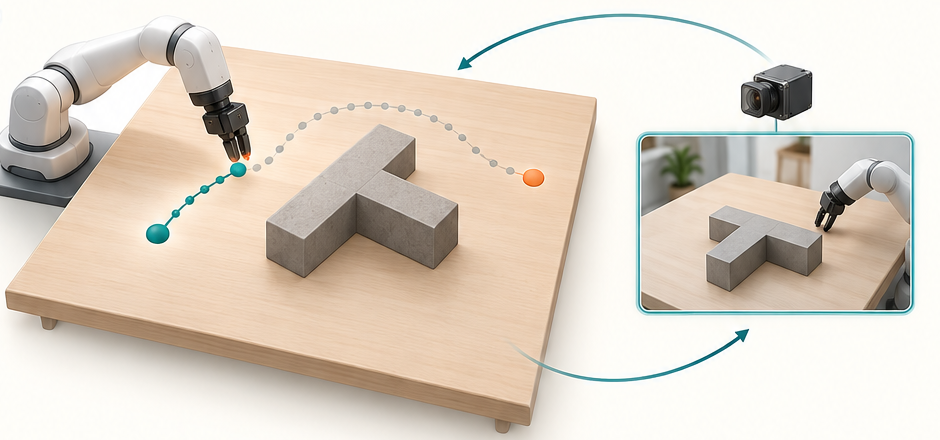
\includegraphics[width=8.0cm]{control-art.png}};
\node at(5.5,2.2){只执行前 $T_a$ 步，刷新 $O_{t+T_a}$ 后重算};
\node at(5.5,1.45){实机 Push-T：$T_o=2,\ T_p=16,\ T_a=6$};
\node[font=\fontsize{10}{13}\selectfont]at(5.5,.75){§I 提问 → II/III A/B/C机制 → IV/V/VI D证据 → VII/VIII定位};
\end{tikzpicture}\end{document}